\documentclass{beamer}

\usepackage[orientation=landscape,size=a0,scale=1.4,debug]{beamerposter}
\mode<presentation>{\usetheme{mlr}}

\usepackage[sfdefault]{roboto}
\usepackage{roboto-mono}
\usepackage[T1]{fontenc}
\usepackage[utf8]{inputenc} % UTF-8
\usepackage[english]{babel} % Language
\usepackage{hyperref} % Hyperlinks
\usepackage{ragged2e} % Text position
\usepackage[export]{adjustbox} % Image position
\usepackage[most]{tcolorbox} % Code boxes
\usepackage{multido}

\hypersetup{
	hyperfootnotes=false,
	colorlinks=true,
	linktocpage=true,
	pdfauthor={mlr-org team},
	%linkcolor=[RGB]{3,99,142}, % mlr blue
	urlcolor=[RGB]{231,138,69}
}

\title{Feature Selection with mlr3fselect :\,: CHEAT SHEET} % Package title in header, \, adds thin space between ::

\newlength{\columnheight} % Adjust depending on header height
\setlength{\columnheight}{84cm} 

\newtcolorbox{codebox}{%
	sharp corners,
	leftrule=0pt,
	rightrule=0pt,
	toprule=0pt,
	bottomrule=0pt,
	fontupper=\robotomono\small,
	hbox}

\newtcolorbox{codeboxmultiline}[1][]{%
	sharp corners,
	leftrule=0pt,
	rightrule=0pt,
	toprule=0pt,
	bottomrule=0pt,
	fontupper=\robotomono\small,
	#1}

\newtcolorbox{codeboxexample}{%
	sharp corners,
	leftrule=0pt,
	rightrule=0pt,
	toprule=0pt,
	bottomrule=0pt,
	fontupper=\robotomono\small,
	width=27cm,
	adjusted title=Example,
	fonttitle = \bfseries\Large,
	top = 0.5em}

\newtcolorbox{codeboxinline}{%
	sharp corners,
	leftrule=0pt,
	rightrule=0pt,
	toprule=0pt,
	bottomrule=0pt,
	hbox,
	nobeforeafter,
	fontupper=\robotomono\small,
	tcbox raise base}

\newcommand{\codeinline}[1]{\begin{codeboxinline}#1\end{codeboxinline}}
\newcommand{\sectionheading}[1]{{\color{mlrblue}\large\raggedright\textbf{#1}}\vspace{1em}}
\newcommand{\monospace}[1]{\multido{}{#1}{\space}}

\begin{document}
\begin{frame}[fragile]{}
	\begin{columns}
		\begin{column}{.245\textwidth}
			\begin{beamercolorbox}[center]{postercolumn}
				\begin{minipage}{.98\textwidth}
					\parbox[t][\columnheight]{\textwidth}{
						\begin{myblock}{Class Overview}
							The package provides a set of R6 classes which allow to (a) define general
							feature selection instances and (b) run algorithms which optimize on these.
							(a) is called a FSelectInstanceSingleCrit or FSelectInstaneMultiCrit, which define a blackbox optimization function that maps feature subsets to resampled performance values for arbitrary performance measures.\\
							\\
							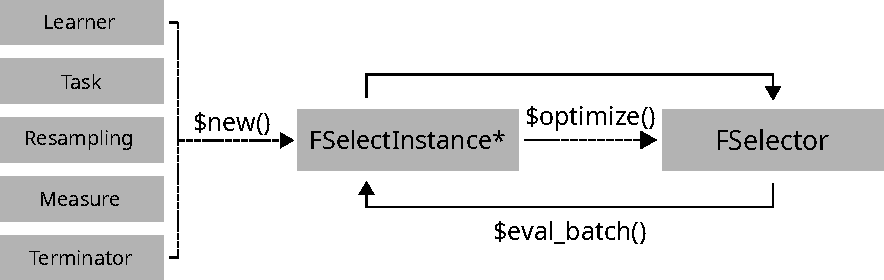
\includegraphics[width=0.95\textwidth]{img/class_diagram.pdf}
						\end{myblock}
						\begin{myblock}{Terminators - When to stop}
						Construction: \codeinline{\textbf{trm}(.key, ...)}
						\\
						\begin{itemize}
							\item \codeinline{evals}
							(\codeinline{n\_evals})\\
							After a given amount of iterations.
							\item \codeinline{clock\_time}
							(\codeinline{secs}, \codeinline{stop\_time})\\
							After a given absolute time.
							\item \codeinline{model\_time}
							(\codeinline{secs })\\
							After a given training time.
							\item \codeinline{perf\_reached}
							(\codeinline{level})\\
							After a specific performance was reached.
							\item \codeinline{stagnation}
							(\codeinline{iters}, \codeinline{threshold})\\
							After the performance stagnated for given iterations.
							\item \codeinline{stagnation\_batch}
							(\codeinline{n}, \codeinline{threshold})\\
							After the performance stagnated for given batches.
						\end{itemize}
						\vspace{1em}
						\begin{codebox}
							as.data.table(\textbf{mlr\_terminators})
						\end{codebox}
						Lists all available terminators.
						% \begin{codebox}
						% 	terminator = term("\textbf{combo}", terminators, any)
						% \end{codebox}
						% List of \codeinline{terminators} that terminate
						% if any (\codeinline{any = TRUE})
						% or all (\codeinline{any = FALSE}) terminators are positive.
					\end{myblock}
						\vfill}
				\end{minipage}
			\end{beamercolorbox}
		\end{column}
		\begin{column}{.245\textwidth}
			\begin{beamercolorbox}[center]{postercolumn}
				\begin{minipage}{.98\textwidth}
					\parbox[t][\columnheight]{\textwidth}{
						\begin{myblock}{FSelectInstance* - Search Scenario}
							Evaluator and container for resampled performances of feature subsets.
							The main (internal) function \codeinline{eval\_batch(xdt)} calls \codeinline{benchmark()} to evaluate a table of feature subsets. 
							Also stores archive of all evaluated feature subsets and the final result.
							\\
							\begin{codeboxmultiline}[width=25cm]
								instance = \textbf{FSelectInstanceSingleCrit}\$new(\\
								\hspace*{1ex}task, learner, resampling, measure,\\
								terminator)
							\end{codeboxmultiline}
							Set \codeinline{store\_benchmark\_result = TRUE} to store resamplings of evaluations and \codeinline{store\_models = TRUE} to store associated models.\\
							\begin{codeboxexample}
								{\scriptsize
									instance = FSelectInstanceSingleCrit\$new(\\
									\hspace*{1ex} tsk("iris"), lrn("classif.rpart"), rsmp("cv"),\\ 	\hspace*{1ex} msr("classif.ce"), trm("evals"))\\
									fselector = fs("random\_search")\\
									fselector\$optimize(instance)}
							\end{codeboxexample}
							Use \codeinline{FSelectInstanceMultiCrit} for multi-criteria tuning.
						\end{myblock}
						\begin{myblock}{FSelector - Search Strategy}
						Feature Selection strategy. 
						Generates feature subsets and passes these to \codeinline{FSelectInstance*} for evaluation until termination.
						Creation: \codeinline{\textbf{fs}(.key, ...)}
						\\
						\begin{itemize}
							\item \codeinline{random\_search}
							(\codeinline{batch\_size})\\
							Random search.
							\item \codeinline{exhaustive\_search}
							(\codeinline{max\_features})\\
							Exhaustive Search.
							\item \codeinline{sequential}
							(\codeinline{strategy})\\
							Sequential Selection.
							\item \codeinline{rfe}
							(\codeinline{feature\_fraction}, \codeinline{recursive})\\
							Recursive Feature Elimination.\\
							\item \codeinline{design\_points}
							(\codeinline{batch\_size }, \codeinline{design})\\
							User supplied feature subsets.
						\end{itemize}
						\vspace{1em}
						\begin{codebox}
							as.data.table(\textbf{mlr\_fselectors})
						\end{codebox}
						Lists all available feature selection algorithms.
					\end{myblock}
						\vfill}
				\end{minipage}
			\end{beamercolorbox}
		\end{column}
		\begin{column}{.245\textwidth}
			\begin{beamercolorbox}[center]{postercolumn}
				\begin{minipage}{.98\textwidth}
					\parbox[t][\columnheight]{\textwidth}{
					
						\begin{myblock}{Executing the Feature Selection}
							\begin{codebox}
								fselector\$\textbf{optimize}(instance)
							\end{codebox}
							Starts the feature selection. \codeinline{FSelector} generates feature subsets and passes these to the \codeinline{\$eval\_batch()} method of the \codeinline{FSelectInstance*} until the budget of the \codeinline{Terminator} is exhausted.
							\\
							\begin{codebox}
								instance\$archive\$\textbf{data()}
							\end{codebox}
							Returns all evaluated feature subsets and their resampling results.
							\\
							\begin{codeboxmultiline}[width=27cm]
								{\tiny
								instance\$archive\$data()\\
								 \#\#\monospace{4}Petal.Length Petal.Width Sepal.Length Sepal.Width classif.ce\monospace{3}uhash\\
							     \#\# 1:\monospace{8}TRUE\monospace{8}TRUE\monospace{9}TRUE\monospace{8}TRUE\monospace{6}0.053  23b...
								 \#\# 2:\monospace{7}FALSE\monospace{8}TRUE\monospace{9}TRUE\monospace{8}TRUE\monospace{7}0.042  45c...
								}
							\end{codeboxmultiline}
							\vspace{1em} 
							\codeinline{uhash} refers to \codeinline{\footnotesize 	{instance\$archive\$benchmark\_result}}.\\
							\begin{codebox}
								instance\$\textbf{result}
							\end{codebox}
							Returns data.table with optimal feature subset and estimated performance.
							\\
							\begin{codebox}
								{\footnotesize task\$select(instance\$\textbf{result\_feature\_set})}
							\end{codebox}
							Set optimized feature subset in \codeinline{Task}.
						\end{myblock}
						\begin{myblock}{AutoFSelector - Select before Train}
						Wraps learner and performs integrated feature selection.
						\\
						\begin{codeboxmultiline}[width=24.5cm]
							at = \textbf{AutoFSelector}\$new(\\
							\hspace*{1ex}learner, resampling, measure, \\
							\hspace*{1ex}terminator, fselector)
						\end{codeboxmultiline}
						\vspace{0.5em}
						Inherits from class \codeinline{Learner}.
						Training starts feature selection on the training set.
						After completion the learner is trained with the "optimal" feature subset on the given task.
						\\
						\begin{codeboxmultiline}[width=16.5cm]
							at\$\textbf{train}(task)\\
							at\$\textbf{predict}(task, row\_ids)
						\end{codeboxmultiline}
					\end{myblock}
						\vfill}
				\end{minipage}
			\end{beamercolorbox}
		\end{column}
		\begin{column}{.245\textwidth}
			\begin{beamercolorbox}[center]{postercolumn}
				\begin{minipage}{.98\textwidth}
					\parbox[t][\columnheight]{\textwidth}{
						\begin{myblock}{Nested Resampling}
							Resampling the \codeinline{AutoFSelector} results in nested resampling with an inner and outer loop.
							\\
							\begin{codeboxexample}
								{\tiny
									resampling\_inner = rsmp("holdout")\\
									evals20 = trm("evals", n\_evals = 20)
									\vspace{1em}
									\\
									at = AutoFSelector\$new(learner, resampling\_inner, \\
									\hspace*{1ex}measure, evals20, fselector) \\
									at\$store\_fselect\_instance = TRUE
									\vspace{1em}
									\\
									resampling\_outer = rsmp("cv", folds = 2)\\
									rr = resample(task, at, resampling\_outer, \\
									\hspace*{1ex}store\_models = TRUE)
									\vspace{1em}
									\\
									as.data.table(rr)\\
									\#\# ...\monospace{8}learner\monospace{5}resampling iteration
									\monospace{13}prediction\\
									\#\# ... <AutoFSelector> <ResamplingCV>\monospace{9}1\monospace{5}<PredictionClassif>\\
									\#\# ... <AutoFSelector> <ResamplingCV>\monospace{9}2\monospace{5}<PredictionClassif>}
							\end{codeboxexample}
							\vspace{1em}
							\begin{codebox}
								rr\$\textbf{aggregate()}
							\end{codebox}
							Aggregates performances of outer folds.
							\\
							\begin{codebox}
								\footnotesize{as.data.table(rr)\$learner[[1]]\$\textbf{fselect\_result}}
							\end{codebox}
							Retrieves inner feature selection results.
							\vspace{-0.5em}
						\end{myblock}
						\begin{myblock}{Logging and Parallelization}
							\begin{codebox}
								{\scriptsize
									lgr::get\_logger("\textbf{bbotk}")\$set\_threshold("<level>")}
							\end{codebox}
							Change log-level only for mlr3fselect.\\
							\begin{codebox}
								future::\textbf{plan}(strategy)
							\end{codebox}
							Sets the parallelization backend.
							Speeds up feature selection by running iterations in parallel.
						\end{myblock}
						\vfill}
				\end{minipage}
			\end{beamercolorbox}
		\end{column}
	\end{columns}
\end{frame}
\end{document}
